\documentclass{article}
\usepackage{graphicx} 
\usepackage{subfiles}
\usepackage{natbib}
\usepackage{hyperref}
\setlength{\bibhang}{0.5in}
\bibliographystyle{apalike}
\usepackage{float}

\title{Tool Demo: Evaluating News Source Trustworthiness with NewsGuard for Misinformation Research}

\begin{document}
\maketitle

\section{Introduction}
On social media, misinformation is widely visible \citep{lazerScienceFakeNews2018} and embedded in growing partisan sorting and inter-group conflict~\citep{gonzalez-bailonAsymmetricIdeologicalSegregation2023a}. 
To study these dynamics on digital platforms, it is imperative for computational communication scientists to have access to reliable and valid tools that enable them to identify misinformation. 
A common approach is to assess the trustworthiness of sources rather than individual pieces of content. 
NewsGuard has emerged as the most widely used database for source ratings \citep{celadinDisplayingNewsSource2023, guessExposureUntrustworthyWebsites2020a, lasserSocialMediaSharing2022c, pratelliSwingingStatesDoes2023, robertsonUsersChooseEngage2023a} and is especially popular in misinformation research for its comprehensive source-level trustworthiness scores, which are compiled based on web tracking data and rated and updated by professional editors and journalists.
Given the popularity of the NewsGuard database as a tool to quantify the prevalence of misinformation, an in-depth analysis of the temporal stability of ratings and the completeness of the database for different countries is warranted.
Furthermore, NewsGuard requires a license, and researchers in need of a measurement instrument to quantify misinformation must weigh the advantages and disadvantages of source-based methods and the investment required to access the NewsGuard database. 
With the present in-depth analysis of the database's content, we aim to provide researchers with the necessary information to make this decision.
We provide recommendations for effectively utilizing the NewsGuard database and source-based approaches alongside our analysis of the content of the database.

\section{NewsGuard: A Popular Database for Source Ratings}
The organization \href{https://www.newsguardtech.com/}{NewsGuard} offers the most comprehensive list of news domains \citep{linHighLevelCorrespondence2023a}. 
It does not just provide a blacklist of untrustworthy sources but provides a trustworthiness score for each source, covering news sources across the entire spectrum of news quality. 
A trained team of experts, mainly consisting of journalists and editors, regularly judges the trustworthiness of the selected news sources based on nine journalistic criteria that are universally applied across countries\footnote{\href{https://web.archive.org/web/20240131155450/https://www.newsguardtech.com/ratings/rating-process-criteria/}{https://www.newsguardtech.com/ratings/rating-process-criteria/}}.
The trustworthiness score is a composite score of these nine indicators: each criterion has a weight, which comprises the overall trustworthiness rating (ranging from 0 to 100). 
Since the overall score is a sum of the individual scores for each criterion, it is not truly continuous, as some values (for example, 1, 2, 3, or 4 points) cannot be achieved by any combination of criteria.
Figure \ref{fig:trustworthiness_panel}B shows the multi-modal structure, indicative of the quasi-continuous nature of the overall NewsGuard score.

\begin{figure}[H]
    \centering
    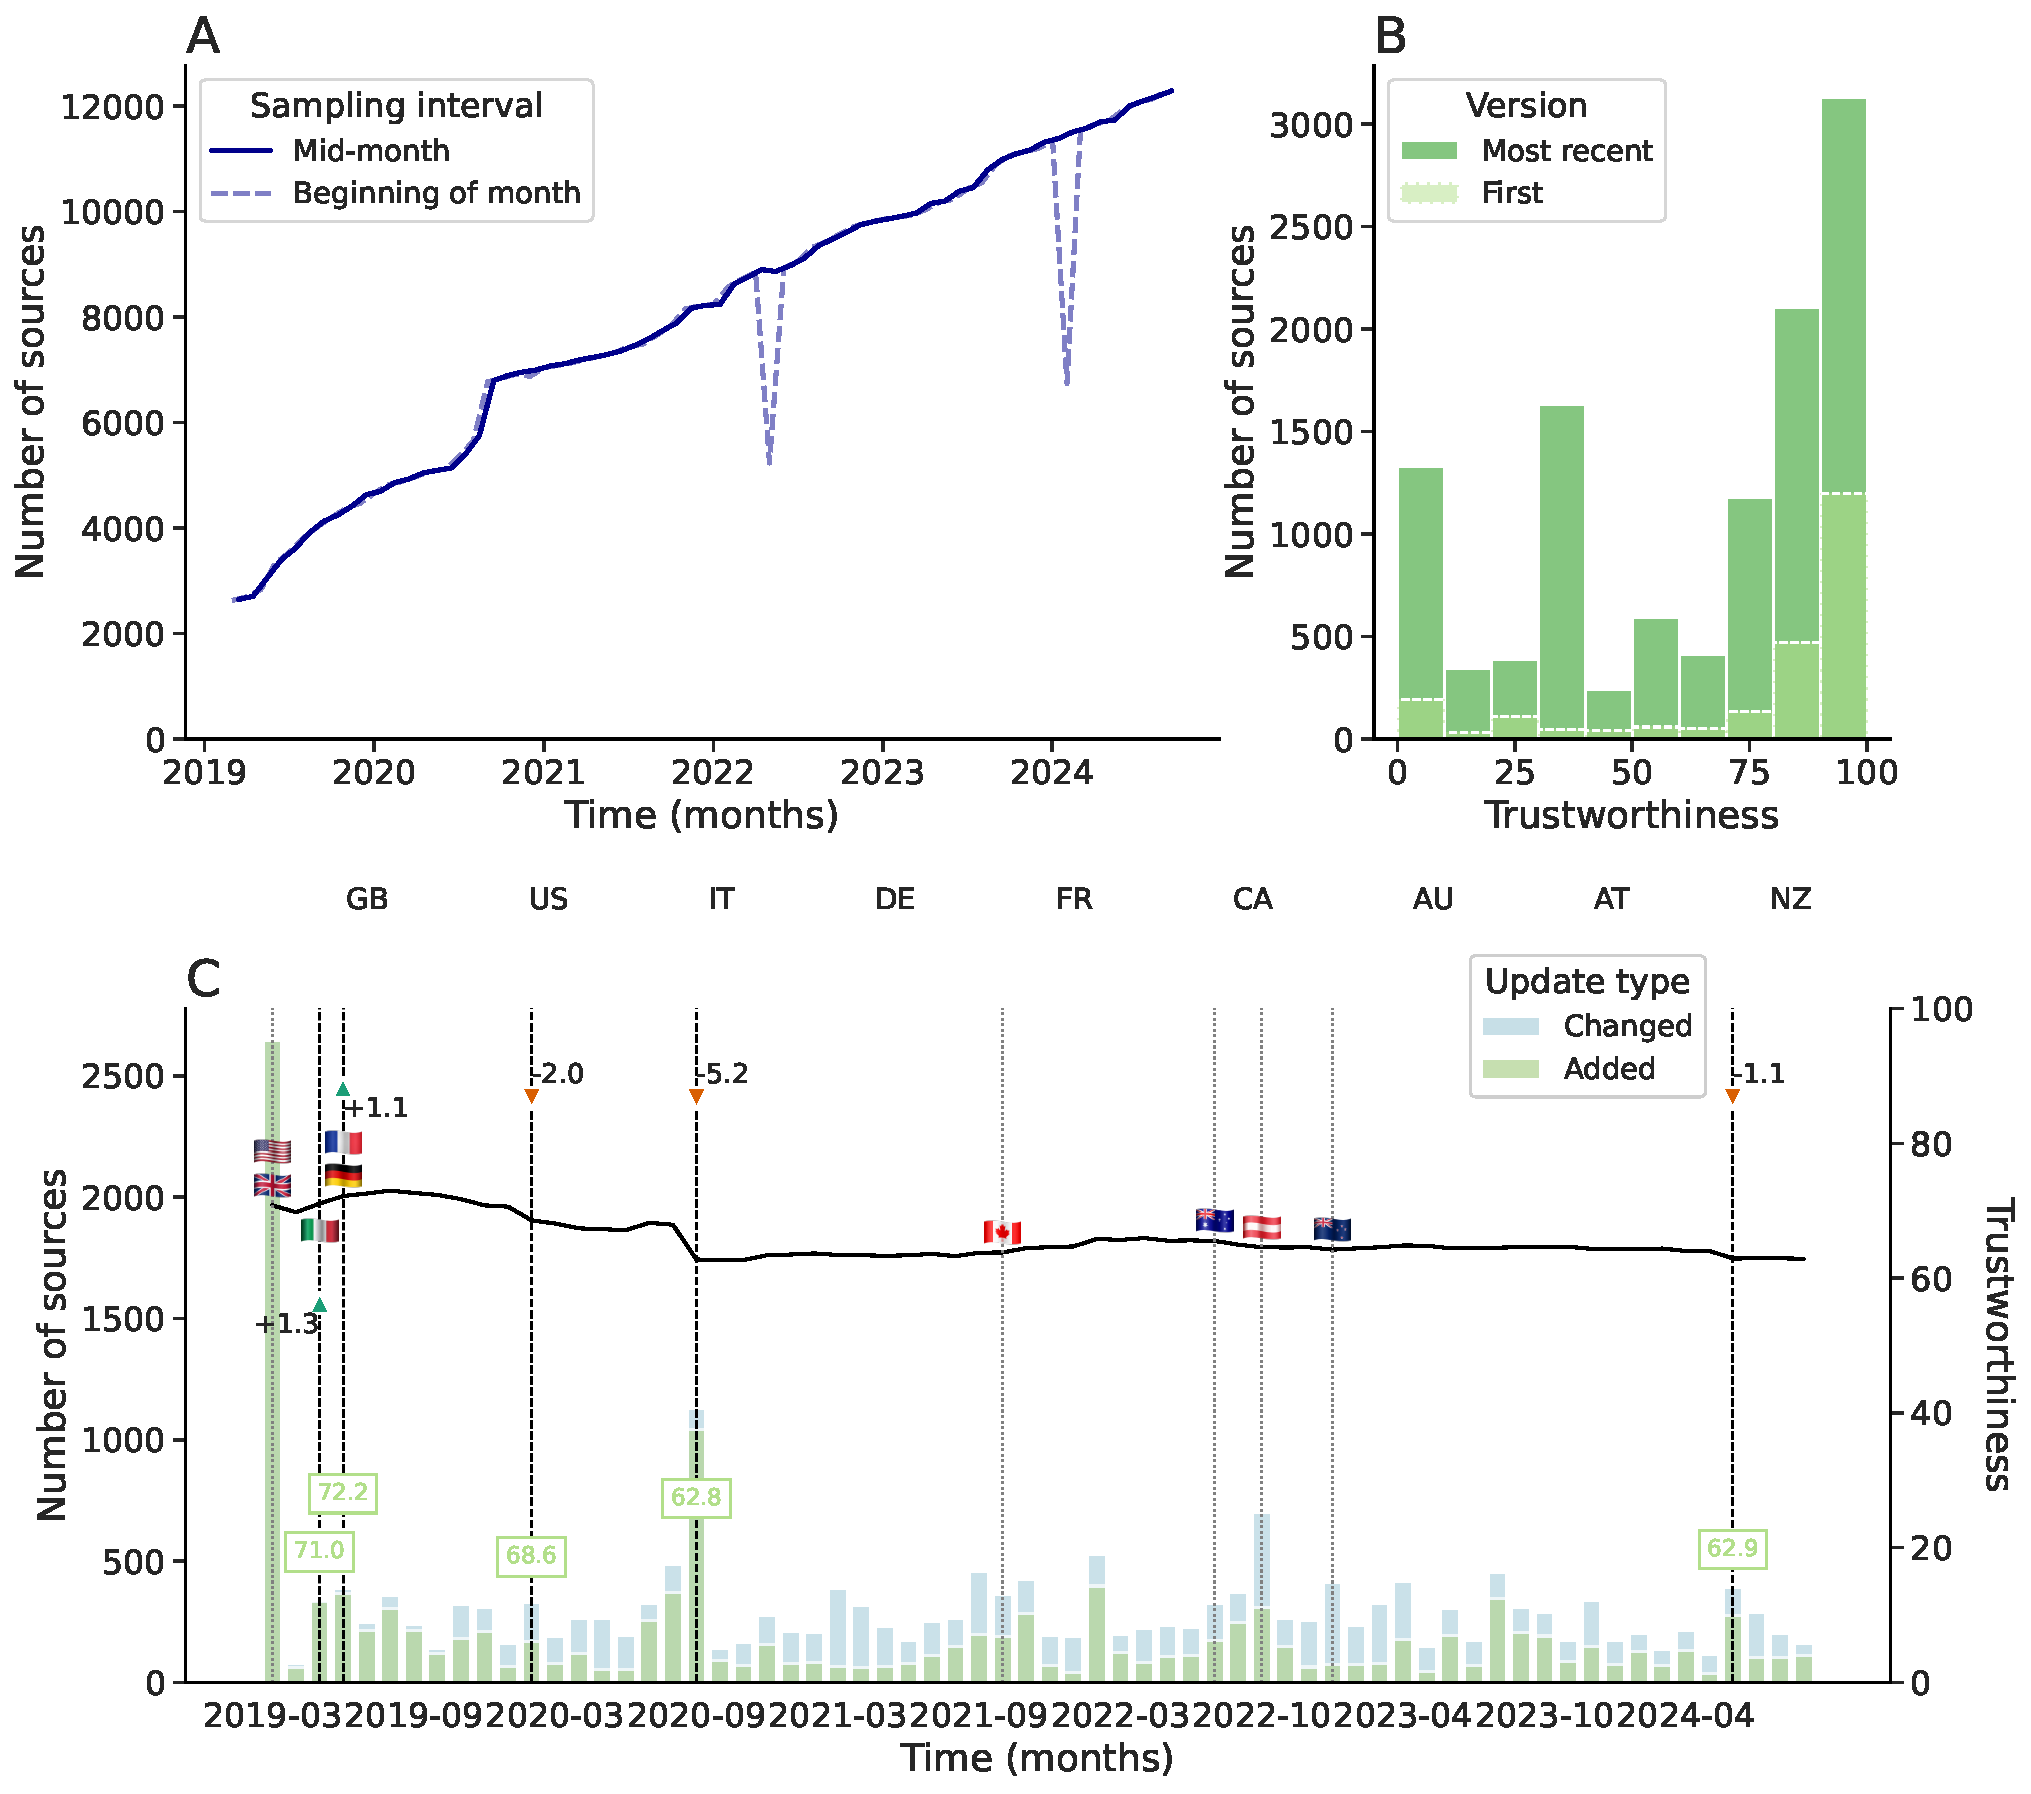
\includegraphics[width=\textwidth]{figures/trustworthiness_panel.pdf}
    \caption{Description of trustworthiness ratings with A showing the number of sources with rating over time based on two different sampling strategies: when sampling one snapshot of the database mid-month (solid line), we observe a steady increase, whereas sampling at the beginning of the month results in two irregular dips (dashed line). Panel B: distribution of trustworthiness in the first and most recent database as a histogram. Panel C: changes in trustworthiness scores over time (monthly granularity), with flags (respective country codes in order of appearance) and dotted lines indicating when countries were added and vertical lines highlighting the top five updates (i.e., major score changes, also shown with arrows). The height of the bars describes the number of sources added vs. changed, with colors indicating the proportions. Note: We include the average trustworthiness of sources added in green for the major changes. Countries are listed in the order added at the top of panel C.}
    \label{fig:trustworthiness_panel}
\end{figure}

NewsGuard curates the list of sources it rates by tracking online activity, claiming to have reviewed news sources accounting for 95\% of online engagement, including news consumed and shared online.
The organization also manually adds sources they deem influential, or that changed their web domain.
NewsGuard regularly updates the database, adding new sources and adjusting ratings based on shifts in journalistic practices, political context, and source ownership.
The database has grown significantly since 2019, expanding from an initial U.S. focus to include sources from the U.K., Canada, Germany, France, and Italy, among others. 
Figure \ref{fig:trustworthiness_panel}A and Figure \ref{fig:trustworthiness_panel}B highlight this growth, showing an increase from approximately 2,375 to over 12,000 entries, with a marked rise in new sources in response to events such as the COVID-19 pandemic. 
The dataset (2019-2024) contains sources from nine countries in total (United States, Great Britain, Italy, Canada, France, Germany, Austria, Australia, and New Zealand; also see Figure \ref{fig:trustworthiness_panel}C) plus sources considered to be global.

As of September 15, 2024, the database has 12,288 entries in total, some without a trustworthiness rating (7.6\%). 
This includes 70 sources classified as a ``platform'' (e.g., YouTube), 63 sources judged as ``satire'' (e.g., The Onion) and 806 lifestyle sources (e.g., healthquote-free.com). 
For the remaining 11,349 sources, the database includes the following characteristics:
\begin{itemize}
    \item Unique identifier for each rating and date of the last update
    \item Domain name and parent domain (e.g., nytimes.com)
    \item A trustworthiness rating as a quasi-continuous scale (between 0 and 100) and binary labels (N = Not Trustworthy/T = Trustworthy) based on a threshold at 60
    \item Language and country associated with the source
    \item Political orientation of the source (e.g., ``left'' and ``right'')
    \item Topics covered (e.g., ``local news'', ``political news'', ``health information'') by the source
\end{itemize}


\section{Descriptive Analysis}
This study examines NewsGuard’s utility for misinformation research by analyzing data from 2019 to 2024. 
Our analysis focused on three primary dimensions: (1) the temporal stability of trustworthiness ratings across different snapshots of the database, (2) the coverage of countries, particularly other than the US, and (3) the usefulness of contextual labels, such as political orientation and topics, for misinformation research.

To examine rating stability, we compared the trustworthiness scores of sources in database snapshots taken over five years. 
As Figure \ref{fig:trustworthiness_panel}C shows, the rating distribution has remained relatively consistent over time.
In fact, close to 60\% of sources have an overall rating of over 60 (see Fig. \ref{fig:trustworthiness_panel}B for the distribution of trustworthiness scores in the most recent vs. the first version of the database).
Overall, the decrease in the overall trustworthiness of sources we can see in Figure~\ref{fig:trustworthiness_panel}C can be attributed to NewsGuard adding untrustworthy sources rather than previously trustworthy sources losing points. 
This finding is supported by changes in journalistic quality criteria during updates (presented in Fig.~\ref{fig:criteria_panel}A).
The most common change is sources stopping disclosing ownership and financing, accounting for 12.3\% of the observed changes.
This indicates either that NewsGuard frequently checks criteria related to ownership or that adherence to such criteria is more volatile. 

Further, such differences in the journalistic criteria per country explain the overall lower trustworthiness score in the US, visible in Figure~\ref{fig:criteria_panel}C.
Figure~\ref{fig:criteria_panel}B shows the percentage of sources that \emph{do not fulfill} a given indicator by country, i.e., a high percentage indicates that many sources fail to meet the criterion.
For most countries, more than 50\% of sources meet each criterion. 
Interestingly, over 70\% of Italian sources do not provide names of content creators, and over 80\% do not effectively correct errors. 
A similar but less pronounced pattern is visible for French sources. 
Across all criteria, the US shows the highest percentage of sources not fulfilling the criteria, with 56.4\% of sources failing to gather and present information responsibly (and 30\% fail to fulfill the heavily-weighted criterion ``Does not repeatedly publish false or egregiously misleading content''), almost twice the share of sources than in any other country.

\begin{figure}[H]
    \centering
    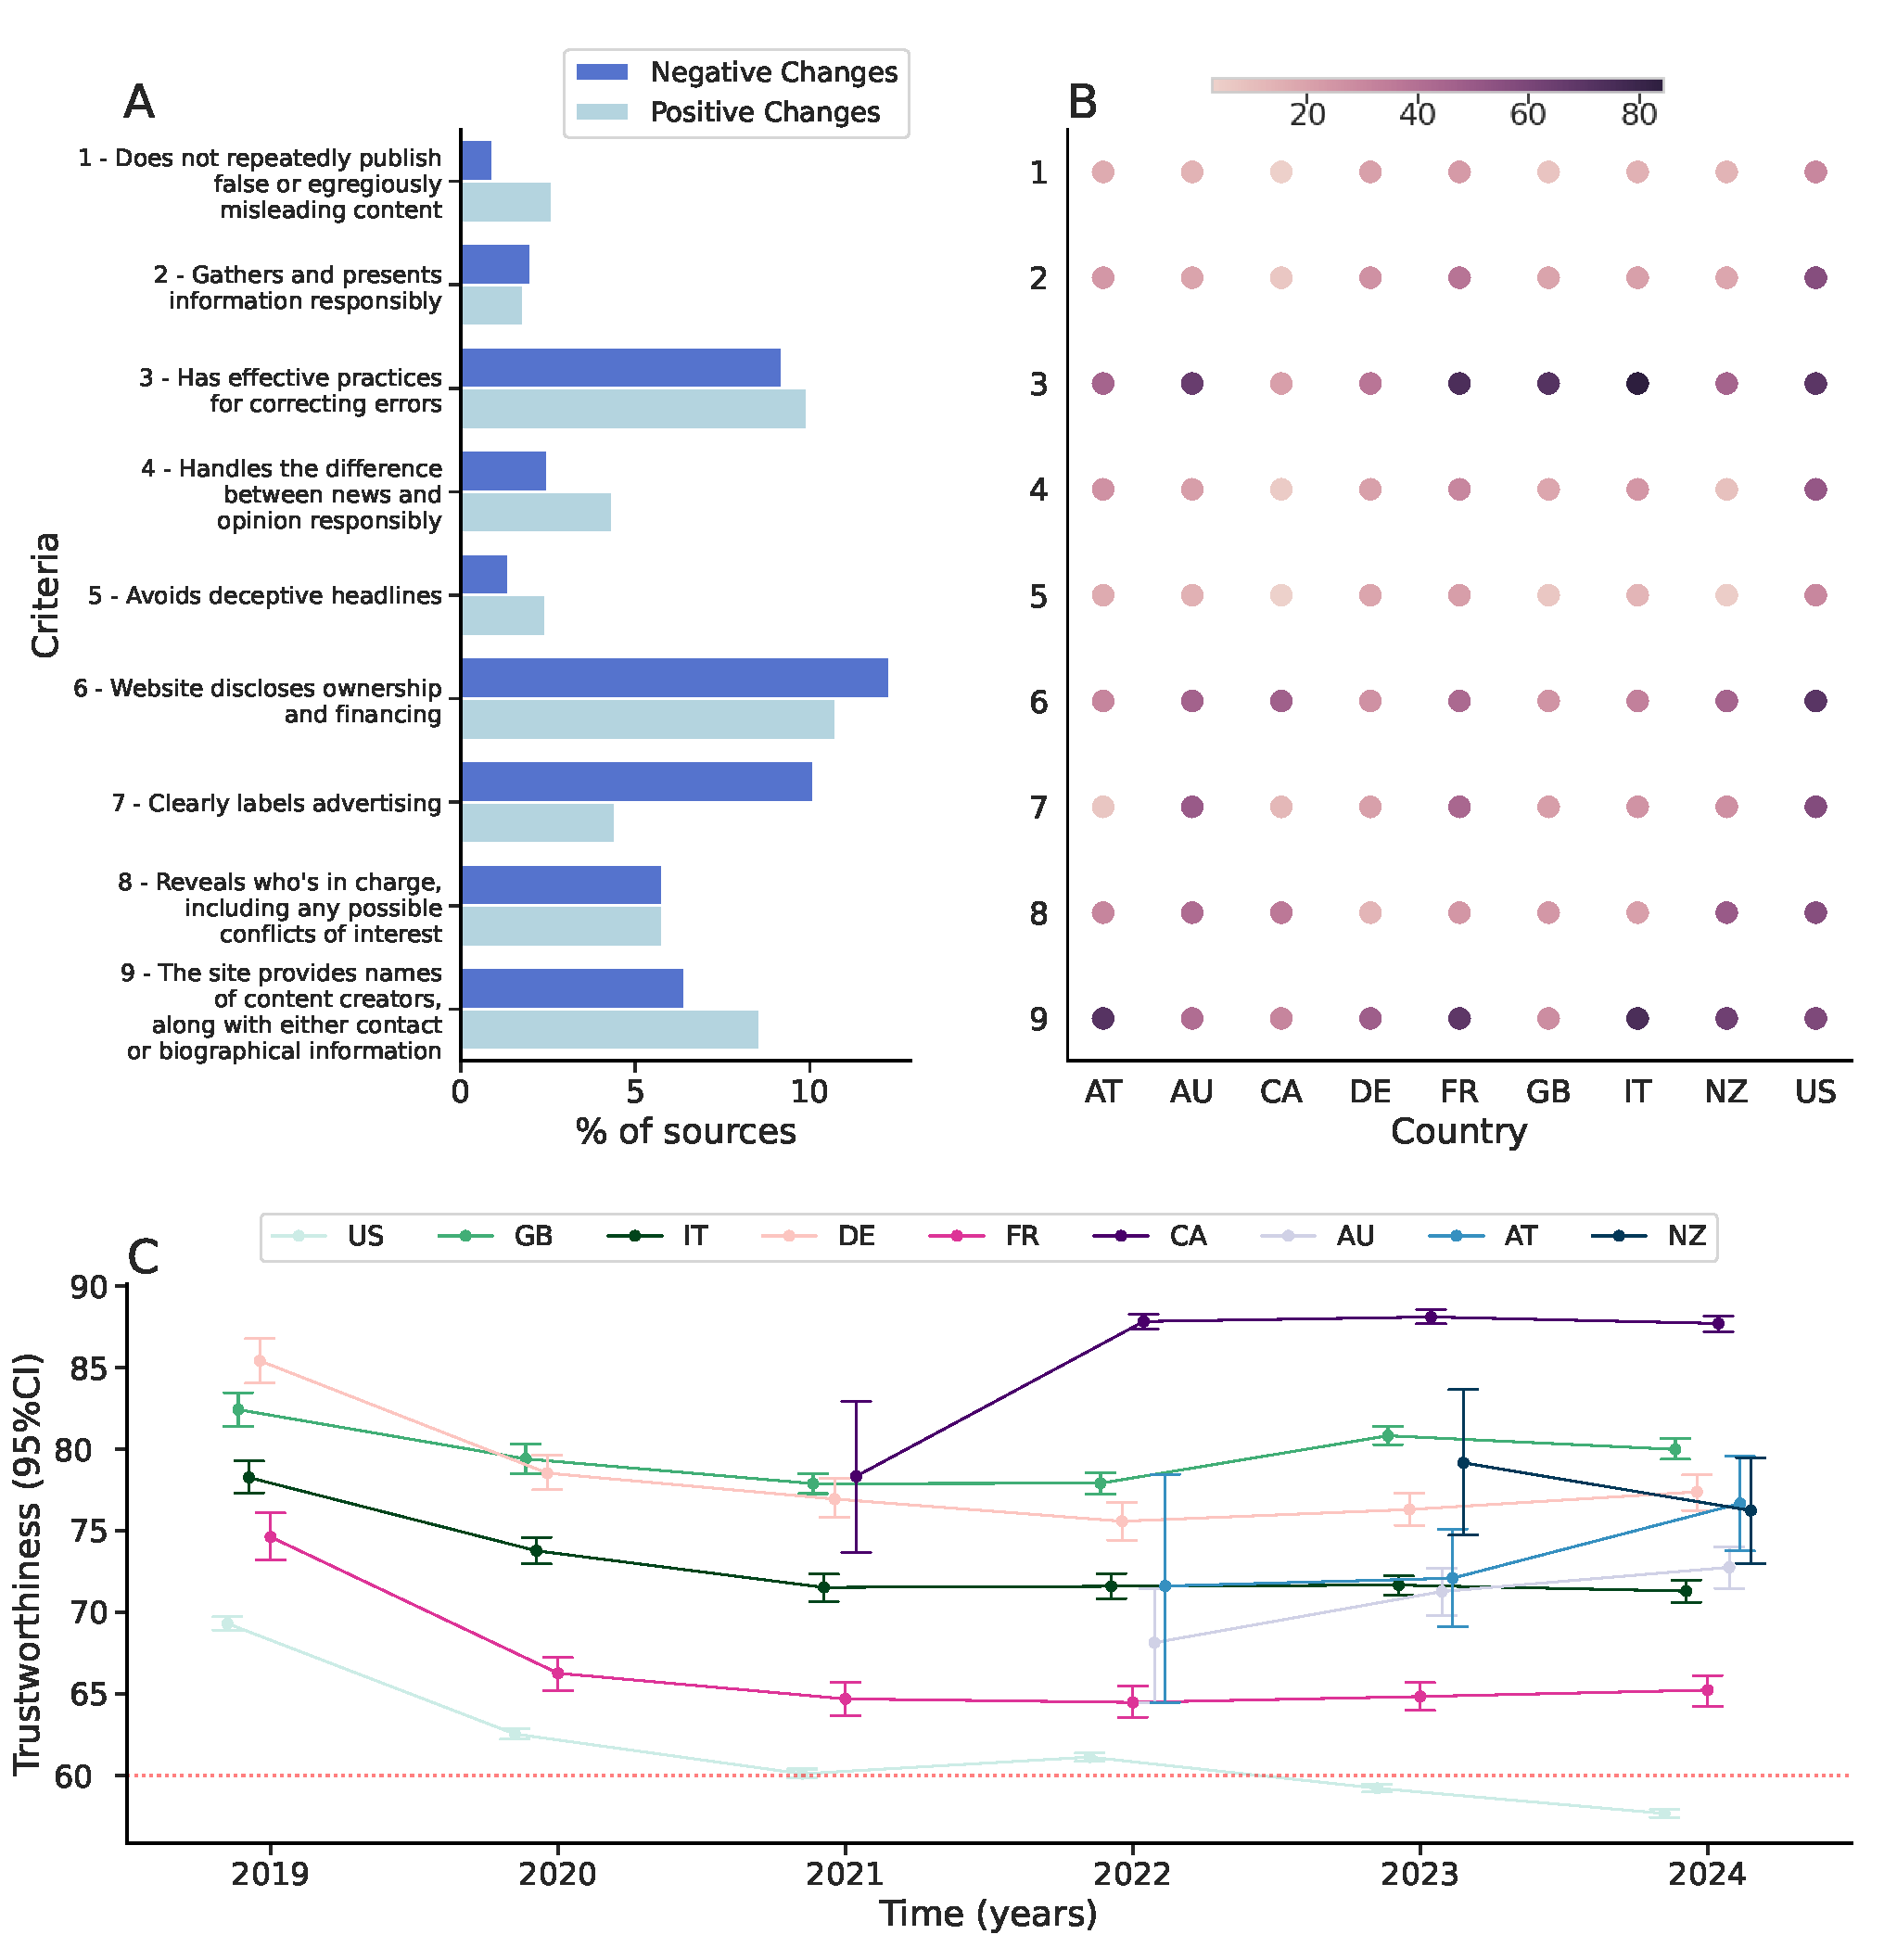
\includegraphics[width=\textwidth]{figures/criteria_panel_cropped.pdf}
    \caption{Panel A: percentage of sources that have stopped or started to fulfill a criterion, including multiple changes (positive vs. negative) of a single source. Panel B: percentage of sources that do not fulfill a criterion per country (July 15th, 2024). Panel C: trustworthiness per country over time (truncated to range from 55 to 90), aggregated per year with 95\% confidence intervals.}
    \label{fig:criteria_panel}
\end{figure}

Additionally, we provide an exemplary reproduction of published research by \cite{lasserSocialMediaSharing2022c} using NewsGuard ratings from different points in time to assess the degree to which results vary based on changes in the measurement instrument.
This analysis highlights consistency across U.S., U.K., and German sources, indicating that research results relying on NewsGuard would not be significantly affected by different database versions. 
We also assessed the completeness of the database by comparing NewsGuard to two lists of frequently shared web domains for the US \citep{linHighLevelCorrespondence2023a} and German context \citep{puschmannGermanOnlineNews2023}.
This comparison reveals that NewsGuard effectively captures widely shared sources, though gaps remain in coverage for certain non-U.S. contexts.

Another key finding relates to NewsGuard’s contextual labels, including political orientation and topic labels.
In December 2022, the political orientation categories were condensed from four to two (see Fig. \ref{fig:orientation_panel}A). 
Overall, the political orientation label is only available for a minority of the sources, specifically 33.4\% (3,789 sources) in the current database version.
These labels, as illustrated in Figure \ref{fig:orientation_panel}B\&C, reveal trends in the trustworthiness of sources based on political alignment.
Across countries, right-leaning sources score lower on average than left-leaning ones, reflecting a pattern observed in previous misinformation research, where right-wing sources are more likely to promote unverified information. 
We manually validated the political orientation labels for German-speaking sources and found high agreement (83\%). 
Our findings suggest two (not necessarily mutually exclusive) implications for a missing political orientation: Either the sources have no overt political bias in their reporting or are too niche to be labeled by NewsGuard.

\begin{figure}[H]
    \centering
    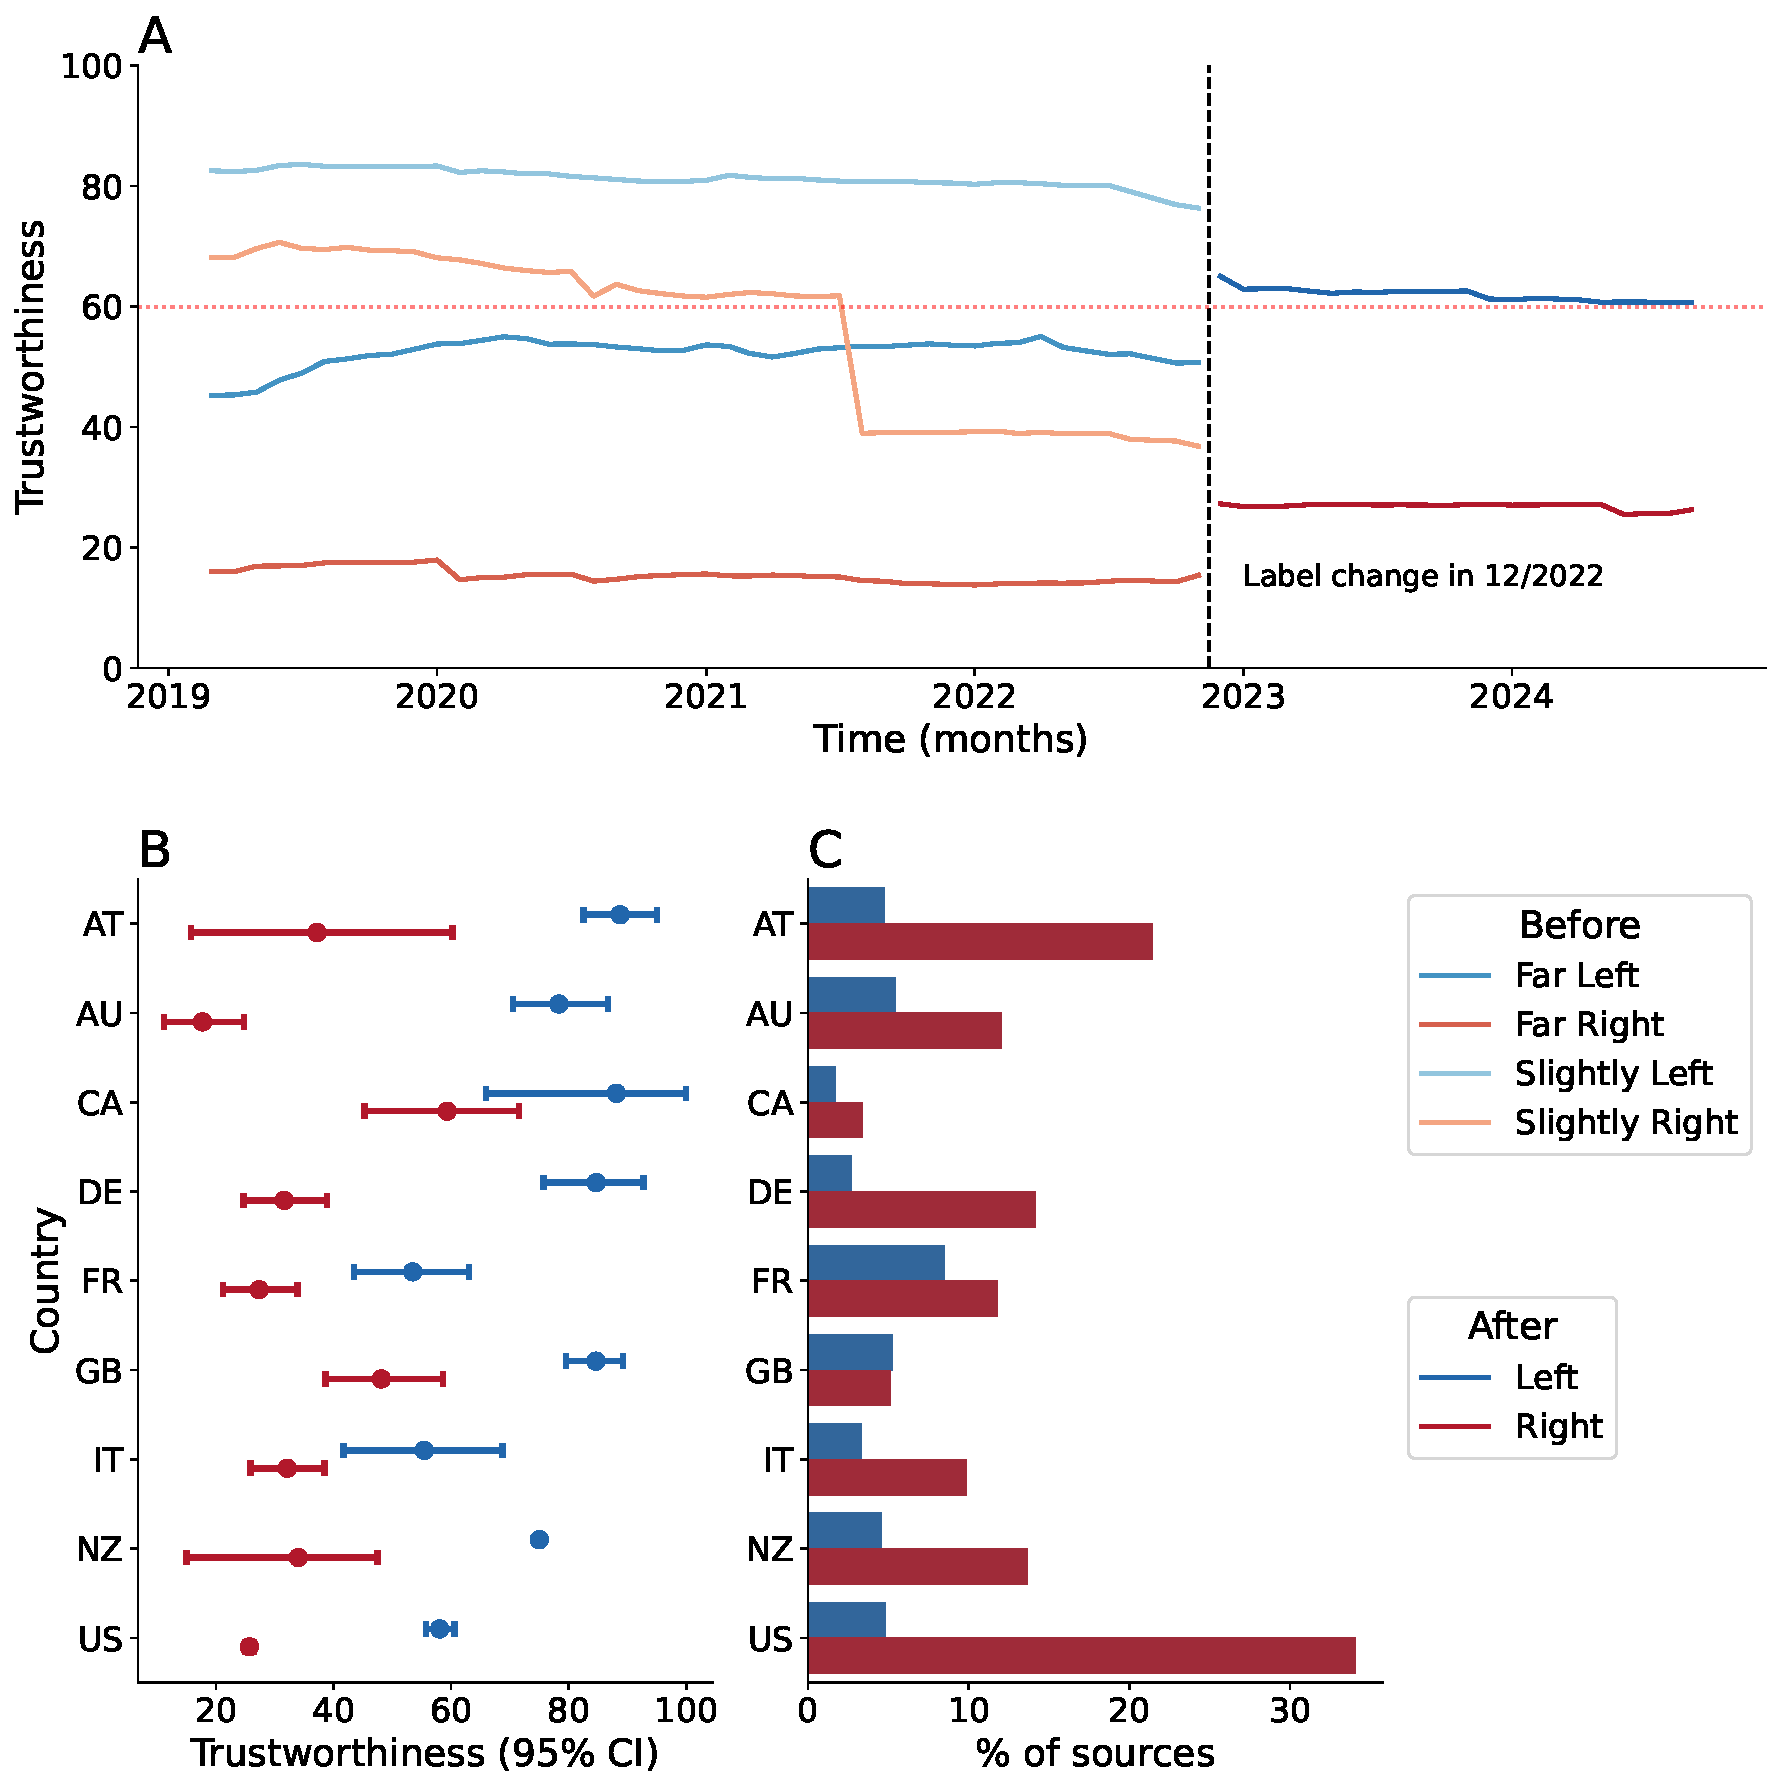
\includegraphics[width=\textwidth]{figures/orientation_panel.pdf}
    \caption{Trustworthiness averages by political orientation. Panel A: over time. Panel B: by country. Panel C: percentage of sources per country with political orientation, explaining differences in trustworthiness by country.}
    \label{fig:orientation_panel}
\end{figure}

Topic labels, which indicate whether sources cover health news, political commentary, conspiracy theories, or general news, also provide critical insights into misinformation trends (Fig. \ref{fig:topics_panel}A, B, \&C shows variations by topic).
As shown in Figure \ref{fig:topics_panel}A, average trustworthiness ratings greatly differ across topics and political orientation (white dots show the average trustworthiness of sources covering that topic).
Overall, the coverage of topic labels appears comprehensive (see Fig. \ref{fig:topics_panel}B for overall counts and Fig. \ref{fig:topics_panel}C for misinformation-related topics), suggesting they could be a valuable asset for misinformation research.

\begin{figure}[htbp]
    \centering
    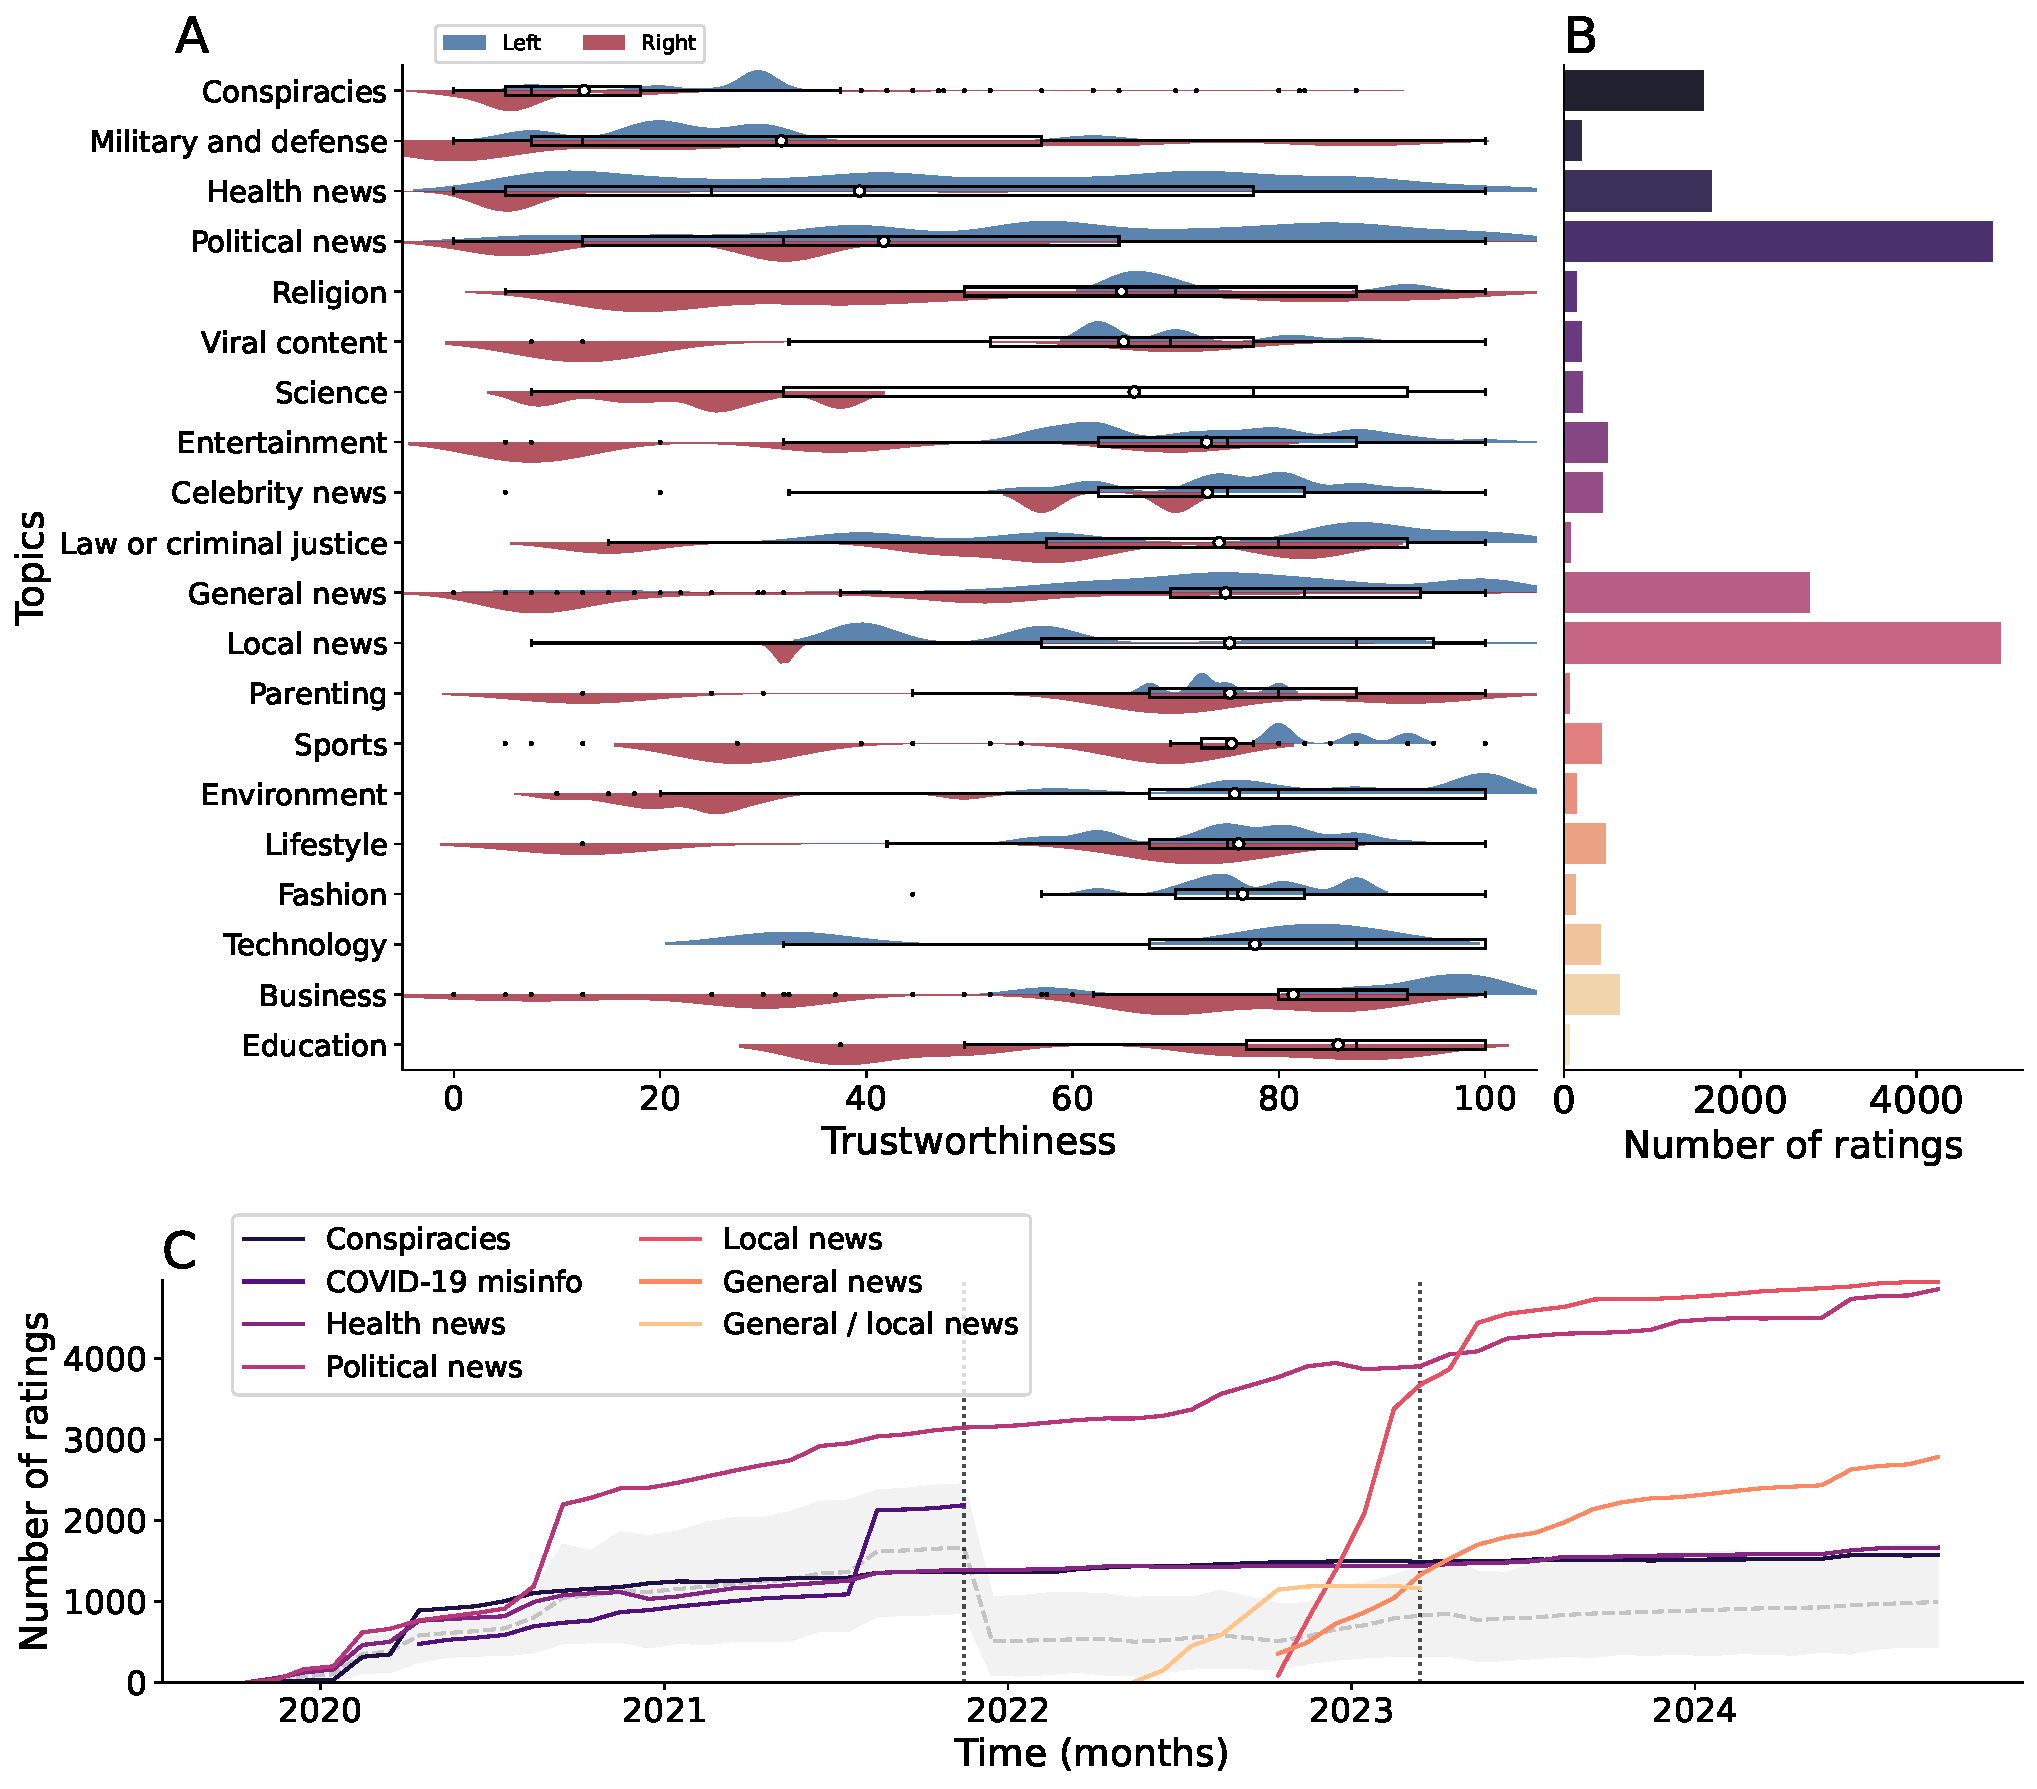
\includegraphics[width=\textwidth]{figures/topics_panel.pdf}
    \caption{A) shows the distributions of trustworthiness per topic and political orientation (left/right in blue/red, respectively), sorted by their average trustworthiness (white dot within the boxplot that represents the quartiles and whiskers show the whole range). 
    Note: We excluded topics with a count below 50. Some topics are abbreviated. B) gives the count of topics as of September 15th, 2024.
    C) shows the frequency of misinformation-related labels over time.
    Colored lines show the top five topics covered by untrustworthy sources. 
    The dotted, vertical lines show the removal of two of those labels.
    The grey and dashed line shows the average topic label count of those topics across all sources with the 95\%CI.}
    \label{fig:topics_panel}
\end{figure}

\section{Practical Recommendations}
This contribution presents best practices on using NewsGuard and source-based approaches generally.
Here, we summarize practical recommendations when using NewsGuard:

First, our analysis shows that NewsGuard’s ratings are generally stable, especially for established countries like the U.S. and Germany, and trustworthiness ratings rarely experience drastic shifts.
We recommend that researchers using the trustworthiness ratings examine several snapshots of the database to ensure no major source additions or deletions occurred recently. 
For countries included in NewsGuard for longer, e.g., the US, Canada, France, Italy, Germany and the UK, we suggest that researchers use whatever version of the database after 2022 they have access to. 
Using different versions of the database for different portions of any data being analyzed from different time periods does not seem necessary, given the general stability of trustworthiness ratings once a source has been included in the database. 
Despite these nuances, the trustworthiness ratings by NewsGuard appear relatively insensitive to time, speaking for the reliability of source-based approaches.

Second, researchers investigating countries for which sources were only recently added to the database (e.g., New Zealand or Austria) should proceed with caution and invest time to validate the coverage of the database for a given country.
We suggest that researchers always use the most recent version of the database and carefully examine it for differences in coverage for different units of analysis, such as political leaning.

Third, we found differences in journalistic quality criteria per country–––reflecting the respective media system \citep{bruggemannHallinManciniRevisited2014b, hallinComparingMediaSystems2004}.
This finding underscores that applications of the database need to be tailored to individual contexts and that researchers should double-check the relevance of the criteria for the country studied, particularly for comparative studies across multiple countries or specific time frames.

Fourth, our observations highlight the value of using other labels to characterize sources in misinformation studies.
Despite being incomplete, the political orientation labels may be a useful addition to the trustworthiness ratings; however, we recommend (at least) spot-checking the ratings for the specific country in which they intend to use the database, especially for major outlets and mainstream media sources. 
If the research focuses on comparing political bias rather than controlling for it, we advise validating and extending the existing ratings provided by NewsGuard.

Lastly, the topic and journalistic criteria ratings appear stable and may offer valuable context for the analysis of misinformation dynamics.
A combination of political orientation and topic labels could effectively characterize sources and identify untrustworthy sources that address and decontextualize mainstream issues beyond hyper-partisan contexts.
% Especially a combination of trustworthiness and topic labels could complement source characterization, for instance, by distinguishing between fringe sources and those addressing mainstream issues. 
% For sources that lack a label for political orientation, topics may help clarify if a source is genuinely neutral or tends to cover extreme topics low in trustworthiness.

\section{Conclusion}
An inherent challenge in misinformation research lies in how false information is defined and measured. 
A prominent approach for tracking online misinformation is to use a list of sources and their web domains. 
Due to its popularity and limited access, we examined the comprehensive NewsGuard database and analyzed the temporal stability and cross-country completeness of their trustworthiness ratings and other source labels relevant to misinformation research. 
In conclusion, using a list of rated online news domains appears to be a stable method for identifying misinformation online at scale.
A source-based approach with a fine-grained rating scheme based on journalistic quality criteria is particularly valuable and theoretically sound because it can encompass a wide range of sources, including less extreme forms of misinformation, thereby better-reflecting people's information diets. 
While the NewsGuard database serves as a useful tool for tracking online misinformation at the level of the source, researchers should weigh its utility for the studied context against associated costs and consider alternative sources \citep[e.g.,][]{linHighLevelCorrespondence2023a} for comprehensive analysis. 
Our findings underscore the critical need for dynamic, multifaceted, and openly accessible methods to get a clear and robust answer on the impact of misinformation on entire populations.

\section{Data and Code Availability}
The code to reproduce the analysis, excluding the NewsGuard database, which is proprietary, is accessible on \href{https://github.com/julaluehring/newsguard-review-analysis}{Github}.

\bibliography{newsguard-review.bib}

\end{document}